\chapter{Classifier}
To predict, we come up with a \textbf{hypothesis}. A hypothesis is a parametrized function that maps input to output
\begin{equation*}
    y = \func{h}{x ; \theta} , \qquad h \in \CalH, \theta \in \Theta
\end{equation*}
where \(\CalH\) is our \textit{hypothesis class}. We wish to find the parameters \(\theta\) that matches our data well. One way to evaluate how well our hypothesis predicts is to introduce a \textbf{loss function} (or \textit{cost function}), \(\func{L}{a,a_h}\) where \(a,a_h\) are in the output set and the loss function assigns a value to how close our prediction \(a_h\) when the actual value is \(a\). We wish that our hypothesis to have the least loss on new data.
\begin{equation*}
    \func{\CalE}{h} = \dfrac{1}{n'} \sum_{i = n + 1}^{n + n'} \func{L}{\func{h}{x^{(i)} ; \theta }, y^{(i)}}
\end{equation*}
One way to do this is minimize the training error 
\begin{equation*}
    \func{\hat{\CalE}}{h} = \dfrac{1}{n} \sum_{i = 1}^n \func{L}{\func{h}{x^{(i)} ; \theta }, y^{(i)}}
\end{equation*}
There are several types of loss function
\begin{description}
    \item[0-1 Loss]
        \begin{equation*}
            \func{L}{a,a_h} = \begin{cases}
                0 & \text{if} a = a_h \\
                1 & \text{otherwise}
            \end{cases}
        \end{equation*}
    \item[Squared loss]
        \begin{equation*}
            \func{L}{a,a_h} = (a - a_h)^2
        \end{equation*}
    \item[Linear loss]
        \begin{equation*}
            \func{L}{a,a_h} = \abs[a - a_h]
        \end{equation*}
    \item[Asymmetric loss] For example, maybe guessing negative wrong is costlier than guessing positive wrongly, in a binary classification problem.
\end{description}
The model we use, typically, selects \(h\) and we need to minimize the loss (or any other optimization) on the \(\theta\) so that our prediction \textit{fits} the data. To determine a good \(\theta\) we need algorithms, \textit{learning algorithms}. Given a classifier \(h\) we can easily evaluate its performance by testing it on new data. However, to evaluate a learning algorithm we have to first train it on some data and then evaluate the resulting classifier on the testing data. Doing this multiple gives us an estimate of how well the algorithm works. In most cases, we do not have access to a lot of data (we don't now the distribution). In these cases we can re-use data using cross validation 


\begin{algorithm}[H]
    \DontPrintSemicolon
    divide $\CalD$ into $k$ equally sized chunks  $\CalD_1 , \dots , \CalD_k$ \;
    \For{$i= 1 \to k$}{
        train $h_i$ on $\CalD - \CalD_i$\;
        compute $\func{\CalE_i}{h_i}$ on the test data $\CalD_i$\;
    }
    \Return{$\frac{1}{k} \sum_{i = 1}^k \func{\CalE_i}{h_i}$}
    \caption{ cross\_validate $(\CalD , k )$}
\end{algorithm}

\section{Linear classifiers}
A linear classifier has the following form
\begin{equation*}
    \func{h}{x; \theta , \theta_0} = \func{\sign}{\theta^T x + \theta_0} \qquad \theta \in \Reals^d , \theta_0 \in \Reals
\end{equation*}

\subsection{Random linear classifier}
One way to select the parameters \(\theta\) and \(\theta_0\) is to randomly select them and return the best one.

\begin{algorithm}[H]
    \DontPrintSemicolon
    \For{$j= 1 \to k$}{
        $\theta^{(j)} = $Random$(\Reals^d)$ \;
        $\theta^{(j)}_0 = $Random$(\Reals)$ \;
    }
    $j^\ast = \argmin_{\substack{1 \leq j \leq k}} \func{\hat{\CalE}}{\func{h}{x, \theta^{(j)} , \theta^{(j)}_0}}$

    \Return{$(\theta^{(j^\ast)} , \theta^{(j^\ast)}_0)$}
    \caption{ random\_linear\_classifier $(\CalD_n , k )$}
\end{algorithm}

\subsection{Perceptron}
A more intelligent way of finding the parameters is to update when we encounter a mistake. The simplest update rule is the \textbf{perceptron}, which is as follows
\begin{equation*}
    \theta' ,\; \theta_0' \gets \theta + y^{(i)}x^{(i)} ,\; \theta_0 + y^{(i)}
\end{equation*}
This update increase the magnitude of \(y^{(i)}\cdot(\theta^T x^{(i)} + \theta_0)\) as shown below, and hence in enough iterations, the sign will become positive.

\begin{align*}
    y^{(i)}\cdot  \left( \theta^{'T} x^{(i)} + \theta'_0 \right) &= y^{(i)} \left( \theta + y^{(i)} x^{(i)} \right)^T x^{(i)} + y^{(i)} \left( \theta_0 + y^{(i)} \right)\\
    &= y^{(i)} \cdot \left( \theta^T x^{(i)} + \theta_0 \right) + (y^{(i)})^2 \left( \norm[x^{(i)}]^2 + 1 \right)\\
    &=  y^{(i)} \cdot\left( \theta^T x^{(i)} + \theta_0 \right)+ \norm[x^{(i)}]^2 + 1
\end{align*}
however it is not clear how other mistakes will affect the current guess.

\begin{algorithm}[H] \label{algo:perceptron}
    \DontPrintSemicolon
    $\theta = 0 $\;
    $\theta_0 = 0 $\;
    \For{$t= 1 \to T$}{
        \For{$i = 1 \to n$}{
            \If{ $y^{(i)} (\theta^T x^{(i)}) + \theta_0 \leq 0$}{
                $\theta = \theta +  y^{(i)} x^{(i)}$ \;
                $\theta_0 = \theta_0 + y^{(i)} $\;
            }
        }
    }

    \Return{$(\theta , \theta_0)$}
    \caption{ perceptron $(\CalD_n , T )$}
\end{algorithm}


By adding another dimension to our data set we can simplify our prediction to pass through the origin
\begin{align*}
    x'       & = \begin{bmatrix}
        x_1 & \dots & x_n & 1
    \end{bmatrix}, \qquad \theta' = \begin{bmatrix}
        \theta & \theta_0
    \end{bmatrix} \\
    \implies & \theta^{'T} x' = \theta^T x + \theta_0
\end{align*}

Therefore, one can also simplify the \Cref{algo:perceptron} to the following

\begin{algorithm}[H]
    \DontPrintSemicolon
    $\theta = 0 $\;
    \For{$t= 1 \to T$}{
        \For{$i = 1 \to n$}{
            \If{ $y^{(i)} (\theta^T x^{(i)}) + \theta_0 \leq 0$}{
                $\theta = \theta +  y^{(i)} x^{(i)}$ \;
            }
        }
    }

    \Return{$\theta $}
    \caption{ perceptron $(\CalD_n , T )$}
\end{algorithm}

To examine the convergence of the perceptron algorithm we need the following definitions. A dataset \(\CalD_n\) is \textbf{linearly separable -through the origin} if there is some \(\theta\) such that
\begin{equation*}
    y^{(i)} \theta^T x^{(i)} > 0 \quad \forall i
\end{equation*}
and similary it is linearly seperable if there are some \(\theta , \theta_0\) such that 
\begin{equation*}
    y^{(i)} \cdot \left( \theta^T x^{(i)}  + \theta_0 \right) > 0 \quad \forall i
\end{equation*}
The \textbf{margin} of a labeled data point \((x,y)\) with respect to a seperator (hyperplane) \(\theta, \theta_0\) is
\begin{equation*}
    y \cdot \dfrac{\theta^T x +  \theta_0}{\norm[\theta]}
\end{equation*}
which basically quantifies how we \(\theta\) approximates the data point \((x,y)\) in a data set \(\CalD_n\). Also the margin of \(\CalD_n\) w.r.t \(\theta, \theta_0\) is
the minimum of all margins:
\begin{equation*}
    \min_i     y^{(i)} \cdot \dfrac{\theta^T x^{(i)} + \theta_0}{\norm[\theta]}
\end{equation*}

\begin{theorem} [Perceptron convergence theorem]
    If there exists a vector \(\theta^\ast\) such that the margin of database with respect to \(\theta^\ast\) is greater than \(\gamma > 0\) and then norm \(\norm[x^{(i)}] \leq R\) for some \(R\) then perceptron will make at most \(\left(\frac{R}{\gamma} \right)^2\) updates/mistakes.
\end{theorem}

\begin{proof}
    The idea of the proof is to put an increasing lower bound on the cosine of the angle between the \(k_{\cardinalTH}\) update \(\theta^{(k)}\) and \(\theta^{\ast}\). Note that 
    \begin{equation*}
        \func{\cos}{\angle \theta^{\ast} , \theta^{(k)}} = \dfrac{(\theta^{\ast})^T \theta^{(k)}}{\norm[\theta^{\ast}] \norm[\theta^{(k)}]}
    \end{equation*}
    we know that for some \(i\), \(\theta^{(k)} = \theta^{(k - 1)} + y^{(i)} x^{(i)}\), then 
    \begin{align*}
        (\theta^{\ast})^T \theta^{(k)} &= (\theta^{\ast})^T \left(\theta^{(k- 1)} + y^{(i)} x^{(i)} \right) \\
        &=(\theta^{\ast})^T \theta^{(k- 1)}+   y^{(i)} (\theta^{\ast})^T x^{(i)} \\
        &\geq  (\theta^{\ast})^T \theta^{(k- 1)} + \gamma \norm[\theta^{\ast}]\\
        &\geq  k \gamma \norm[\theta^{\ast}]
    \end{align*}
    also 
    \begin{align*}
        \norm[\theta^{(k)}]^2 &=  \left(\theta^{(k- 1)} + y^{(i)} x^{(i)} \right)^T  \left(\theta^{(k- 1)} + y^{(i)} x^{(i)} \right)\\
        &= \norm[\theta^{(k-1)}]^2 + 2y^{(i)} (\theta^{(k-1)})^T x^{(i)} + \left( y^{(i)}\right)^2 \norm[x^{(i)}]^2 \\
        &\leq  \norm[\theta^{(k-1)}]^2 +  \norm[x^{(i)}]^2 \\
        &\leq  \norm[\theta^{(k-1)}]^2 + R^2 \\
        &= kR^2
    \end{align*}
    therefore 

    \begin{equation*}
        \func{\cos}{\angle \theta^{\ast} , \theta^{(k)}} \geq \sqrt{k} \; \frac{\gamma}{R}
    \end{equation*}
    Since the cosine can not exceed one therefore the we at most make 

    \begin{equation*}
        k \leq \left(\dfrac{R}{\gamma}\right)^2 
    \end{equation*}
    mistakes.
 \end{proof}

\section{Features}
\subsection{Transformation}
As we saw we can transform linearly separable dataset to another linearly seperable dataset but without an offset. What happens if the original dataset is not linearly seperable? For example, \textit{xor dataset}:
\begin{figure*}[!ht]
    \centering
    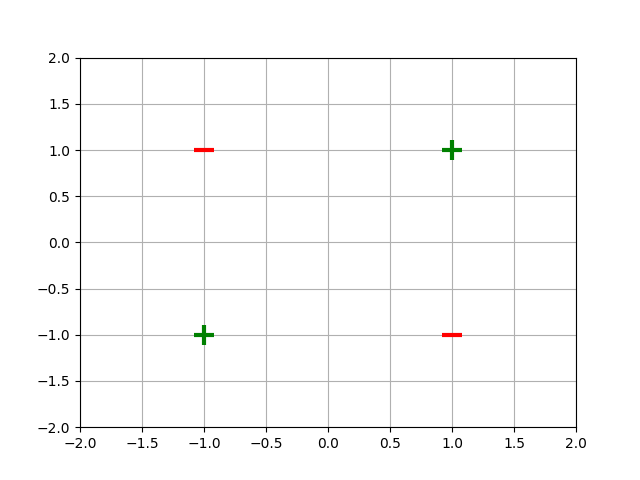
\includegraphics{Chapters/graphics/xor_dataset.png}
    \caption{XOR dataset}
\end{figure*}

\begin{equation*}
    \CalD = \set{((-1,-1),1), ((-1,1), -1) , ((1,-1),-1) , ((1,1),1)}
\end{equation*}
is not linearly seperable in 2 dimensions. A transformation that might be applicable here is \textbf{polynomial basis}. A polynomial basis transformation of order \(k\), transforms a feature \(x \in \Reals^d\) to
\begin{equation*}
    \func{\phi}{x} = ( x_1^{\alpha_1} \dots x_d^{\alpha_d}) , \quad \sum_{i = 1}^d \alpha_i \leq k , \forall i, \alpha_i \geq 0
\end{equation*}
which has \(\binom{k + d }{d }\) dimension.

For example, the transformation \(\func{\phi}{x_1, x_2} = (x_1,x_2,x_1x_2)\) makes the xor dateset linearly seperable-through the origin.
\begin{figure*}[!ht]
    \centering
    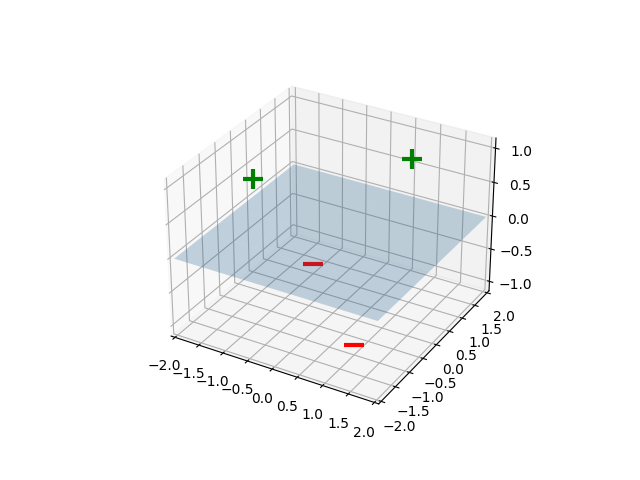
\includegraphics{Chapters/graphics/xor_3d.png}
    \caption{Transformed XOR dataset}
\end{figure*}
\subsection{Representation}
we can represent a discrete feature as
\begin{enumerate}
    \item numeric
    \item thermometer code (a vector of \(m\) booleans where \(1\dots j\) bits are on and the rest or off)
    \item one-hot (a vector of \(m\) booleans where \(j_{\cardinalTH}\) bit is on adn the rest are off)
    \item factoring (group information of a feature based its structure maybe)
\end{enumerate}

For numeric feature we would like to standardized as follow
\begin{equation*}
    \tilde{x_j}  = \dfrac{x_j - \bar{x_j}}{\sigma}
\end{equation*}